\section{Results}
\label{sec:results}

\subsection{Signal level: what each front end removes}

\begin{figure*}[t]
\centering
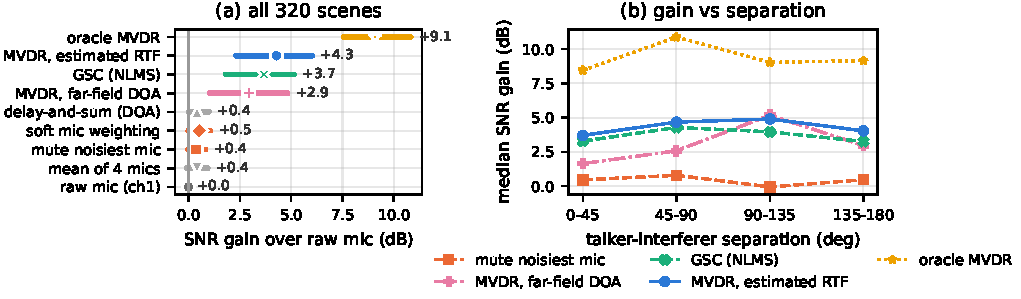
\includegraphics[width=\textwidth]{figures/spatial.pdf}
\caption{Exact SNR gain over the raw microphone (output minus input SNR on
ch1, the same weights applied to the true speech and noise components).
(a) Median and interquartile range over all \NScenes{} scenes. (b) Median
gain against the angle between talker and interferer as seen by the array,
each measured from its own clean take.}
\label{fig:spatial}
\end{figure*}

Figure~\ref{fig:spatial}a ranks the front ends by exact SNR gain.

\paragraph{Muting cannot work.} Switching off the noisiest microphone gains
\Gainmute\,dB and its per-band version \Gainmutesoft\,dB, no more than
simply averaging the four (\Gainmean\,dB). A far-field source reaches four
omnidirectional microphones within 6.4\,cm at the same level, so there is
no ``noisier'' microphone to drop. Delay-and-sum also gives
\Gainds\,dB: at speech frequencies the aperture is a fraction of a
wavelength, so phase alignment alone builds almost no directivity.

\paragraph{MVDR works.} The front ends that whiten the noise do:
\begin{itemize}
\item MVDR with an RTF from covariance whitening: \Gainmvdrrtf\,dB;
\item the adaptive GSC: \Gaingsc\,dB;
\item MVDR steered by the estimated direction: \Gainmvdrdoa\,dB.
\end{itemize}
The oracle MVDR, with the true noise covariance and speech RTF, reaches
\Gainoracle\,dB. That leaves about 5\,dB between what the silence model
supports and what the array could do. The gain holds across separations
(Fig.~\ref{fig:spatial}b), and is lowest when talker and interferer are
within 45$^\circ$ of each other.

\paragraph{Why the DOA-steered MVDR lags.} Its far-field steering depends
on a direction estimate (Fig.~\ref{fig:doa}). With an interferer at
0\,dB, the direction from the mixture minus the silence model is off by a
median \DoaErrSnrZero$^\circ$. At 10\,dB the error falls to
\DoaErrSnrOneZero$^\circ$. Steering by the RTF avoids the question: it
learns the talker's real transfer function, reverberation and near-field
included.

\begin{figure}[t]
\centering
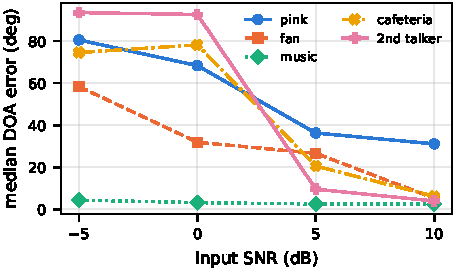
\includegraphics[width=\columnwidth]{figures/doa.pdf}
\caption{Talker direction estimated from the mixture (SRP-PHAT on mixture
minus silence model) against the direction from the clean take.}
\label{fig:doa}
\end{figure}

\subsection{Recognition: the attenuation limit}

\begin{figure*}[t]
\centering
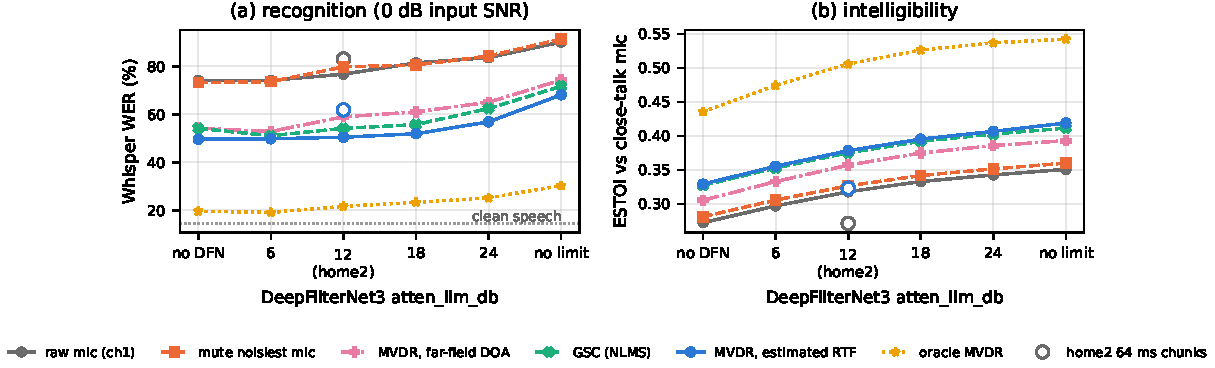
\includegraphics[width=\textwidth]{figures/atten.pdf}
\caption{All 0\,dB scenes (\NDfnScenes), each front end followed by
DeepFilterNet3 at every attenuation limit. (a) Whisper WER against the read
prompt; dotted: the same Whisper on the clean speech-only take. (b) ESTOI
against the close-talk microphone. Hollow markers: the robot's mode, with
independent 64\,ms chunks, at 12\,dB.}
\label{fig:atten}
\end{figure*}

Figure~\ref{fig:atten} shows the central result.

\paragraph{The front end dominates.} Without DeepFilterNet3, Whisper's WER
is \Werrefattoff\,\% on the raw microphone, \Wermuteattoff\,\% with the
mute, \Wergscattoff\,\% with the GSC and \Wermvdrrtfattoff\,\% with the RTF
MVDR. The paired difference against the raw microphone is \DiffRtfVsRef{}
points ($p=$\,\PRtfVsRef, Wilcoxon over scenes). With the oracle the WER is
\Weroracleattoff\,\%, close to the clean floor of \WerClean\,\%.

\paragraph{DeepFilterNet3 does not help the recognizer.} Its effect is the
same on every front end:
\begin{itemize}
\item At 6 and 12\,dB the WER barely moves: \DiffRefDfnTwelve{} and
  \DiffRtfDfnTwelve{} points at 12\,dB, $p=$\,\PRefDfnTwelve{} and
  \PRtfDfnTwelve.
\item From 18\,dB on, the WER rises: without a limit, by \DiffRefDfnInf{}
  and \DiffRtfDfnInf{} points.
\item Meanwhile ESTOI rises monotonically with the limit
  (Fig.~\ref{fig:atten}b).
\end{itemize}
This is the perceptual-versus-recognition split known from enhancement
artifacts~\cite{iwamoto2022artifacts}. For Whisper, the best limit is
``off'' to 12\,dB, and the robot's 12\,dB is at the safe edge.

\paragraph{The robot's chunked mode costs accuracy.} Enhancing each 64\,ms
chunk independently, peak-normalized, adds \DiffRtfHomeTwo{} points after
MVDR ($p=$\,\PRtfHomeTwo) and \DiffRefHomeTwo{} on the raw microphone
($p=$\,\PRefHomeTwo), relative to one continuous pass at the same limit.
The recurrent state of DeepFilterNet3 never warms up, and each chunk is
rescaled on its own.

\begin{figure}[t]
\centering
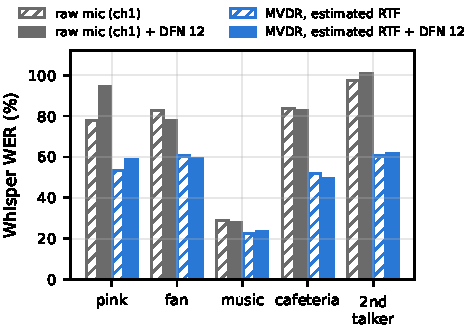
\includegraphics[width=\columnwidth]{figures/noise.pdf}
\caption{WER by interferer at 0\,dB SNR, raw microphone against RTF MVDR,
each without (hatched) and with DeepFilterNet3 at 12\,dB (solid).}
\label{fig:noise}
\end{figure}

\paragraph{By interferer} (Fig.~\ref{fig:noise}):
\begin{itemize}
\item The spatial front end helps most against the second talker
  (\Werrefattofftalker\,\% $\to$ \Wermvdrrtfattofftalker\,\%) and the
  cafeteria (\Werrefattoffcafeteria\,\% $\to$
  \Wermvdrrtfattoffcafeteria\,\%), the two interferers that are speech.
\item DeepFilterNet3 does not help even for stationary pink noise: on the
  raw microphone it raises the WER from \Werrefattoffpink\,\% to
  \WerrefattOneTwopink\,\%.
\item Music is the easiest interferer at equal SNR.
\end{itemize}

\subsection{Live takes}

\begin{figure*}[t]
\centering
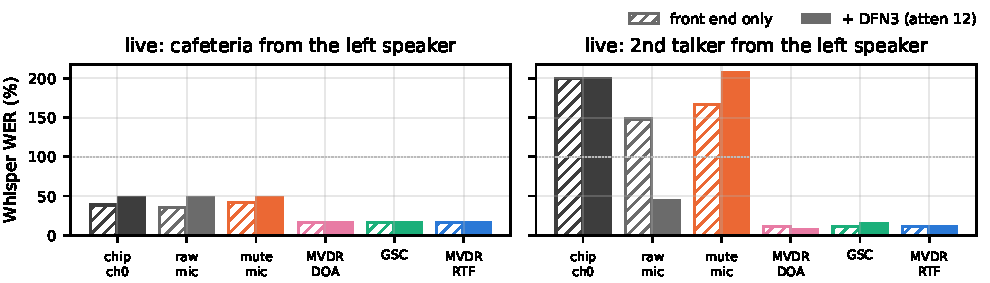
\includegraphics[width=\textwidth]{figures/live.pdf}
\caption{Live takes: the talker reads while an interferer plays from the
left speaker. Hatched: front end only. Solid: followed by DeepFilterNet3
at 12\,dB. ``chip ch0'' is the array's own processed channel, the robot's
current input. WER above 100\,\% means Whisper transcribed the interfering
voice.}
\label{fig:live}
\end{figure*}

\paragraph{Superposition check.} The talker live take replayed the same
interferer samples as its noise-only take. Before the talker speaks, the
live recording matches the scaled noise-only take with a residual of
\SuperResidual\,dB. Most of the residual sits below 300\,Hz, in room noise
that differs between takes. The rest comes from the talker's body and the
changed loudspeaker volume. Subtracting the matched interferer gives the
live speech component, and on it the RTF MVDR gains
\LiveGainmvdrrtf\,dB (DOA-steered: \LiveGainmvdrdoa\,dB; mute:
\LiveGainmute\,dB). These are somewhat below the mixed scenes, as the
residual suggests.

\paragraph{Live recognition} (Fig.~\ref{fig:live}). With an English
talker playing:
\begin{itemize}
\item On the chip's processed channel, with or without DeepFilterNet3,
  Whisper produces a Spanish rendering of the \emph{interfering} voice:
  WER \LivetalkerchZerochipDfn\,\%. The chip's own beam follows the louder
  voice.
\item The raw microphone with DeepFilterNet3 reaches
  \LivetalkerrefDfn\,\%.
\item Every phase-aware front end gets 7--15\,\%. The RTF MVDR followed by
  DeepFilterNet3 gets \LivetalkermvdrrtfDfn\,\%.
\end{itemize}
In the cafeteria take the beamformers reach \LivecafeteriamvdrrtfDfn\,\%,
against \LivecafeteriachZerochipDfn\,\% for the chip channel.
